%!TEX root = ../main.tex
\section{Introduction and IoT Foundations for Connected Vehicles}
\label{sec:introduction}

Modern transportation systems are undergoing a major digital transformation.
As cities grow and vehicle traffic increases, traditional traffic management methods struggle to prevent collisions and reduce road congestion.
To solve these problems, the Internet of Things (IoT) has expanded into the automotive sector, creating the Internet of Vehicles (IoV) \cite{szalay2023survey}.
In this paradigm, vehicles are no longer isolated mechanical machines.
Instead, they act as intelligent mobile IoT devices equipped with computational processors, storage units, multiple wireless radios, and advanced perception sensors.
Within the scope of the Internet of Things (\textit{Internet das Coisas} -- IDC) course at Faculdade de Ci\^{e}ncias da Universidade de Lisboa (FCUL), this survey investigates how foundational IoT paradigms enable cooperative, safe, and autonomous vehicular networks.

The core communication framework of IoV is known as Vehicle-to-Everything (V2X) communication.
V2X enables cars to exchange dynamic information with nearby nodes in real time.

\begin{figure}[!t]
\centering
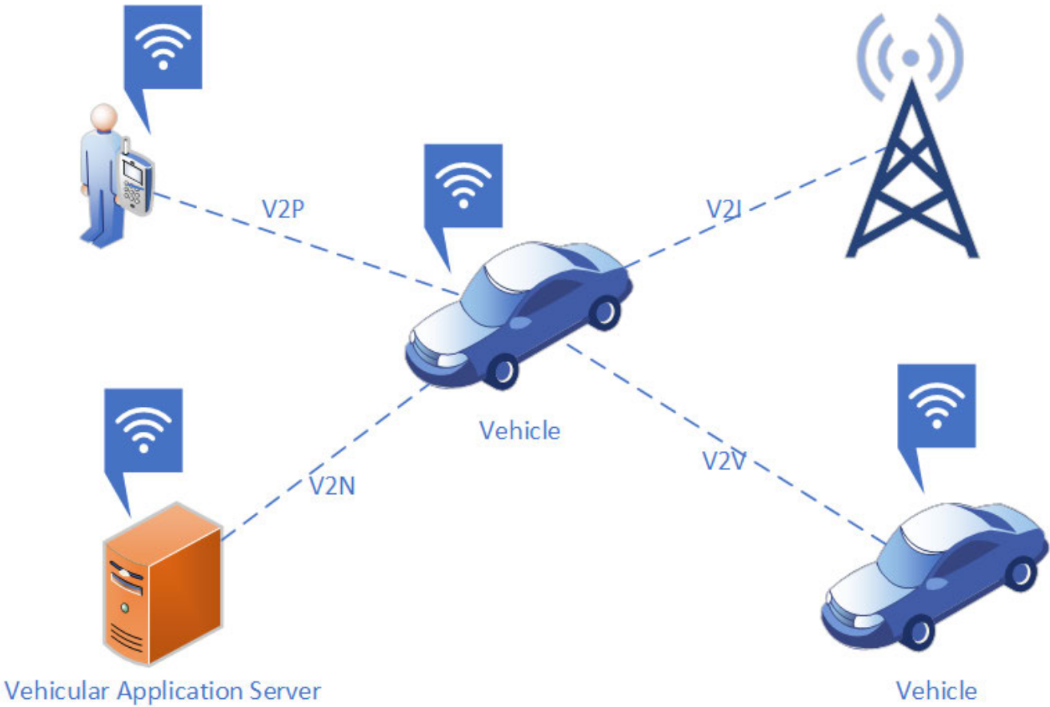
\includegraphics[width=0.88\columnwidth]{figures/rq1/rq1_v2x_communication_modes.png}
\caption{The main communication modes of Vehicle-to-Everything (V2X): V2V, V2I, V2P, and V2N.}
\label{fig:v2x_modes}
\end{figure}

As shown in Fig.~\ref{fig:v2x_modes}, V2X communication is grouped into four distinct interaction types:
\begin{itemize}
    \item \textbf{Vehicle-to-Vehicle (V2V):} Direct communication between vehicles.
    Vehicles broadcast their position, speed, and heading to surrounding cars, enabling active safety features such as forward collision warnings, intersection assistance, and emergency brake lights.
    \item \textbf{Vehicle-to-Infrastructure (V2I):} Communication between vehicles and stationary Roadside Units (RSUs) mounted along streets, intersections, and highways.
    RSUs provide localized speed limits, signal phase and timing (SPaT) information, and warnings about icy roads or nearby construction sites.
    \item \textbf{Vehicle-to-Pedestrian (V2P):} Direct communication with vulnerable road users (VRUs), including pedestrians, cyclists, and road workers equipped with smartphones or wearable tags.
    This link enables pedestrian collision warnings even when a person is hidden behind parked trucks.
    \item \textbf{Vehicle-to-Network (V2N):} Long-range wireless connections between vehicles and cellular base stations or cloud servers.
    V2N provides long-distance traffic navigation, real-time map updates, weather forecasts, and fleet management services.
\end{itemize}

Although modern autonomous vehicles use powerful onboard sensors such as cameras, radar, and LiDAR, operating in isolation has fundamental physical limits.
An onboard sensor cannot see through physical obstacles like buildings, heavy trucks, or sharp corners.
Furthermore, bad weather such as thick fog, heavy rain, or blizzards significantly shortens sensory detection range.
Cooperative V2X communication addresses these limits by allowing vehicles to share what their sensors detect, creating a collective, extended field of view \cite{etsi_cpm_2019}.

However, achieving safe and reliable cooperative driving requires answering three fundamental questions, which form the sequential spine of this survey:
\begin{enumerate}
    \item \textbf{Radio Access Technologies (Section~\ref{sec:technologies_and_deployment}):} How do vehicles transmit safety data wirelessly, and how do dedicated short-range standards compare with cellular technologies in real-world deployments worldwide?
    \item \textbf{Cooperative Perception (Section~\ref{sec:cooperative_perception}):} How can vehicles share their sensor observations to cooperate safely in automated driving, and what are the exact requirements for communication latency and reliability?
    \item \textbf{Security and Privacy (Section~\ref{sec:security_privacy}):} How can we protect vehicular messages against cyberattacks and malicious falsification while preventing adversaries from tracking drivers' daily travel routes?
\end{enumerate}

The remainder of this survey is organized to follow this logical progression.
Section~\ref{sec:technologies_and_deployment} provides a detailed technical comparison of Cellular V2X and IEEE 802.11 standards and surveys their global deployment.
Section~\ref{sec:cooperative_perception} examines cooperative perception architectures, sensor fusion strategies, quality-of-service demands, and failure patterns in simulation.
Section~\ref{sec:security_privacy} investigates vehicular public key infrastructures, pseudonym lifecycles, revocation mechanisms, and key limitations.
Section~\ref{sec:challenges_future} discusses open research challenges in channel congestion, edge computing, misbehavior detection, and the transition toward 6G-V2X.
Finally, Section~\ref{sec:conclusion} concludes the paper with a summary of key insights.
